\chapter{General Introduction to RAG}
\label{chap:General_Introduction_RAG}

\section{General Functioning of LLMs}
Large Language Models (LLMs) are advanced AI systems designed to interact with human language. They operate primarily by predicting the next token (word-pixel...) in a sequence, utilizing massive neural networks trained on vast amounts of text data (Transformers) . However, while they excel at general language tasks, they face critical limitations when handling massive, domain-specific, or highly updated datasets due to strict context window constraints.
\vspace{1cm}
\begin{figure}[h]
    \centering
    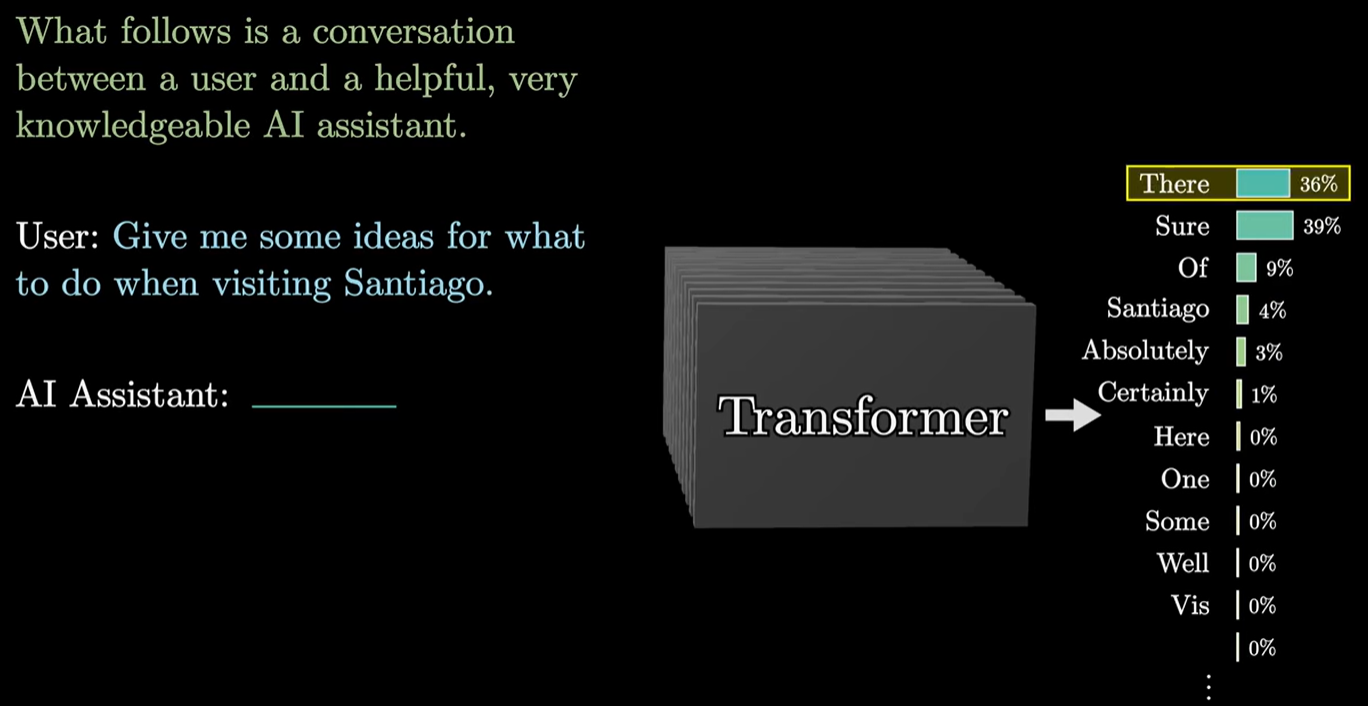
\includegraphics[width=0.8\textwidth]{Figures/Transformer.png}
    \caption{LLM Next Token Prediction }
\end{figure}



\section{Concepts and Fundamentals of RAG}

\subsection{Problem Statement}
In many enterprise scenarios, we possess a large volume of documents and need to use an LLM to answer questions based strictly on that data. The main issue is that standard LLM APIs do not support reading such massive amounts of data at once due to their limited "context window". 

\subsection{The Solution: }
To bypass the context window limitation, we convert our data into vectors and do the exact same for the user's prompt. RAG operates through a core pipeline: it reads the files, improves the prompt by injecting relevant vectors, and finally allows the LLM to create the answer based on that augmented prompt.

\subsection{Search Concepts}
\subsubsection{Traditional Search (Keyword Search)}
Traditional search relies on exact keyword matching to find information within documents. While fast, it often fails to capture the underlying intent if synonyms or different phrasings are used.

\subsubsection{Semantic Search}
Semantic search implies searching for information using its core meaning rather than specific keywords. To achieve this, the system relies on Embeddings.

\subsection{Embeddings}
Embeddings involve transforming words, sentences, or documents into dense numerical vectors within a high-dimensional space. In this representation, each element (dimension) of the vector corresponds to a latent semantic feature or concept, such as "gender," "royalty," or "animacy".

\subsubsection{Origin of Vector Values}
These numerical values are not assigned manually; they are "learned" during the training phase of a Neural Network. 
\begin{itemize}
    \item \textbf{Training Process:} Initially, a model assigns random values to words. As it processes millions of text samples, it adjusts these values based on the "Distributional Hypothesis," which suggests that words appearing in similar contexts share similar meanings.
    \item \textbf{Weights:} The values within the vector are essentially the "weights" of the neural network's hidden layers that have been optimized to capture linguistic patterns.
\end{itemize}

\subsubsection{Vector Dimensionality}
The number of elements in a vector is known as its "dimensionality."some models use  highe dimensions to capture complex nuances:
\begin{itemize}
    \item \textbf{Word2Vec:} Typically uses 300 dimensions.
    \item \textbf{BERT:} Uses 768 dimensions.
    \item \textbf{OpenAI (text-embedding-3-small):} Uses 1,536 dimensions.
\end{itemize}

\subsubsection{Mathematical Relationships and Similarity}
The spatial arrangement of these vectors allows for "vector arithmetic," where semantic relationships are preserved. 
\textbf{Example:}
$$ \text{king} [0.7, 1] \approx \text{woman} [0.1, 0] + \text{royal} [0, 1] - \text{man} $$

\subsection{Vector Databases}
A Vector Database is a specialized type of database where information is saved in the form of multi-dimensional vectors. This architecture allows for rapid semantic search based on meaning by employing efficient indexing algorithms. Popular applications include Chroma (Free, Python-based), Pinecone (Paid), and Weaviate.

\subsection{Indexing Algorithms}
To efficiently search through millions of vectors, Vector Databases use specialized algorithms:
\begin{itemize}
    \item \textbf{HNSW (Hierarchical Navigable Small World):} Uses graphs where each word/vector is connected to its relevant neighbors.
    \item \textbf{IVF (Inverted File Index):} Groups vectors into clusters to speed up the search.
    \item \textbf{LSH (Locality-Sensitive Hashing):} Hashes similar input items into the same buckets with high probability.
\end{itemize}

\subsection{Chunking and Chunking Strategies}
Chunking refers to the method by which we split our large documents into smaller, manageable pieces before vectorization. Common strategies include:
\begin{itemize}
    \item \textbf{Character/Letter based chunking:} Splitting data by a fixed number of characters (e.g., 200-500 or 50-100 characters).
    \item \textbf{Paragraph based chunking:} Splitting data logically by paragraphs to maintain structural context.
    \item \textbf{page based chunking:} Splitting data logically .
    \item \textbf{Zone based chunking:} Splitting data by Zones .
\end{itemize}

\subsection{Caching}
Caching means saving the final answer of an expensive or repetitive computation (or LLM query) so that subsequent identical requests can be answered instantly without repeating the entire RAG process.

\section{RAG Application Architectures}

% --- BASIC RAG ---
\subsection{Basic RAG (Naive RAG)}
Basic RAG follows a straightforward linear pipeline:
1. Convert documents to Embeddings.
2. Embed the user Query.
3. Retrieve similar documents to the query.
4. Augment the prompt with the retrieved documents.
5. Generate the response.
\begin{figure}[h]
    \centering
    % Ensure your file is named 'basic_rag.png' or 'basic_rag.jpg'
    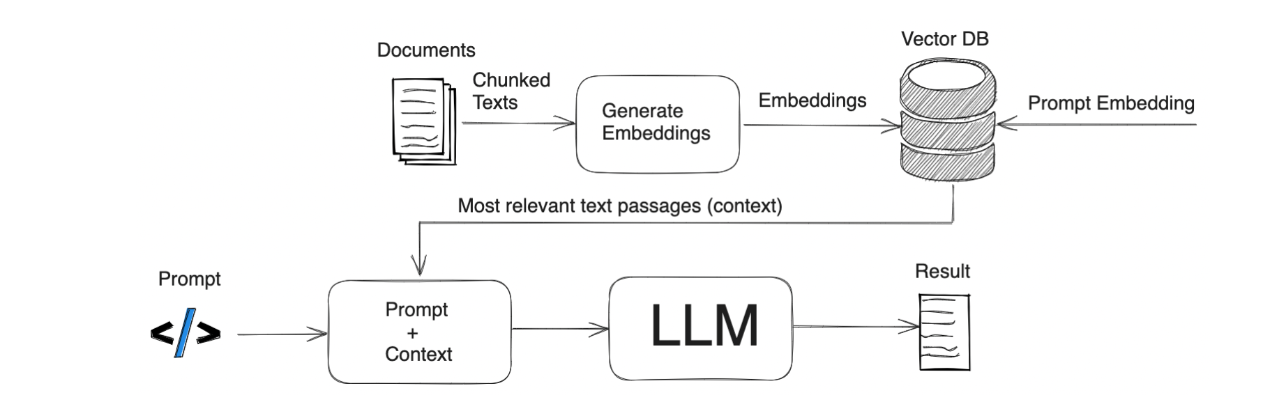
\includegraphics[width=\textwidth]{Figures/BasicRag.png} 
    \caption{Basic RAG Architecture: From Document Embedding to Generation}
\end{figure}

\paragraph{Disadvantages (Limitations):}
\begin{itemize}
    \item \textbf{Equal treatment for Documents:} Relies purely on feature similarity without weighting document authority.
    \item \textbf{Single retrieval step:} Fails on complex queries that contain multiple sub-questions.
    \item \textbf{Lack of query adaptation:} The normal RAG does not differentiate between specific questions and general questions that require reading extensive information.
    \item \textbf{No verification:} If the retrieval step fetches wrong or irrelevant information, the LLM will generate a hallucinated response.
\end{itemize}

% --- ADVANCED RAG ---
\subsection{Advanced RAG}
Advanced RAG builds upon the basic architecture by adding sophisticated filtering and routing mechanisms. It is essentially Basic RAG combined with: Multi-step Retrieval, Dynamic Query Reformulation, Relevance Filtering, and Self-correction mechanisms using specialized architectures.

\paragraph{Examples of Advanced RAG Pipelines Used:}
To solve the limitations of Basic RAG, the industry has developed numerous advanced architectural paradigms. Some of the most notable include:

\begin{itemize}
    \item Cache-Augmented Generation (CAG)
    \item Agentic RAG
    \item Corrective RAG (CRAG)
    \item Self-Reflective RAG
    \item RAG Fusion
    \item Temporal Augmented Retrieval (TAR)
    \item Plan RAG
    \item Graph RAG
    \item Forward-Looking Active REtrieval (FLARE)
    \item Contextual Retrieval
\end{itemize}

\vspace{0.3cm}
\noindent \textbf{Learn More:} For a comprehensive breakdown and technical details of these advanced architectures and retrieval mechanisms, please refer to the official LangChain documentation: \\
\url{https://python.langchain.com/docs/concepts/#retrieval}